% !TeX root = ../main.tex
\section{Design of Compiler}
The compiler is composed of three primary parts, which is explained in the following sections.
The explanation both covers code snippets of the compiler as well as reasoning behind development decisions.
However it is also quite import to address the decisions regarding each component on a larger scale, regarding each phase of the compilation process, also to introduce the components of the compiler before they are explained in depth.
\begin{figure}[H]
	\centering
	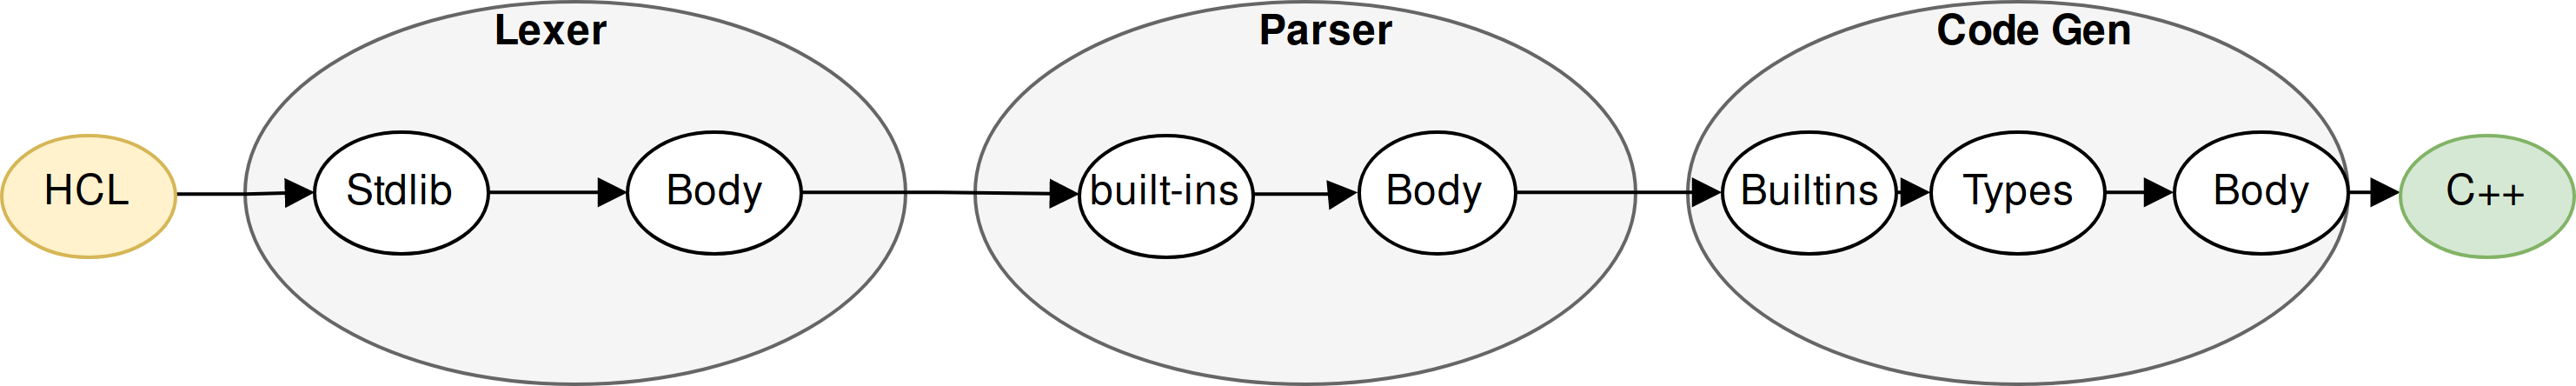
\includegraphics[width=\textwidth]{4.Solution/images/compiler_process.png}
	\caption{The default code when opening ArduinoBlocks}
	\label{fig:compilerProcess}
\end{figure}


The compiler is composed of a lexer, a parser and a code generator, as seen in figure \ref{fig:compilerProcess}.
The lexer generates a token stream from a text stream, which is fed into the parser, which then orders these tokens into an abstract syntax tree.
The abstract syntax tree is then processed by the code generator, which outputs code in our output language, c++.

Some compilers are build with an isolated type checker, however as the HCL language has only predefined types and a relatively simple structure, the type checking happens as part of the parser.

Checking the validity of identifiers also happens in the parser, meaning that this is the largest part of the compiler.
This is done with a symbol table, which are composed of layers, that are created and popped when entering or leaving a scope.
 
As the HCL language has built-in methods, these are hard-coded into the parser, and added to the symbol-table, as the first part of the parsing procedure.

Other compilers would ideally also have an optimization phase, but as the output language is going through another compiler, it is less relevant, as the other compiler is going to optimize the program either way. 
With this in mind more energy have been put into creating a good parser and code generator, than efficiency of the output program.
